% !TEX encoding = UTF-8
% !TEX program = xelatex
\documentclass[12pt,a4paper]{article}
\usepackage[paperwidth=210mm, paperheight=297mm, left=0.75in, right=0.75in, bottom=1in, top=1in]{geometry}
\usepackage{polyglossia}
\setdefaultlanguage[babelshorthands]{italian}
\usepackage{fontspec}
\usepackage{graphicx}
\usepackage{blindtext}
\usepackage{wrapfig}

\frenchspacing
\makeindex

\begin{document}
\title{\vspace{-70pt}Telescopio spaziale AMS}
\author{Giada Frignani}
\date{}
\maketitle
\pagestyle{empty}
\thispagestyle{empty}

\section*{Storia}
\label{storia}
\begin{wrapfigure}{r}{0.35\textwidth}
  \vspace{-10pt}
  \begin{center}
    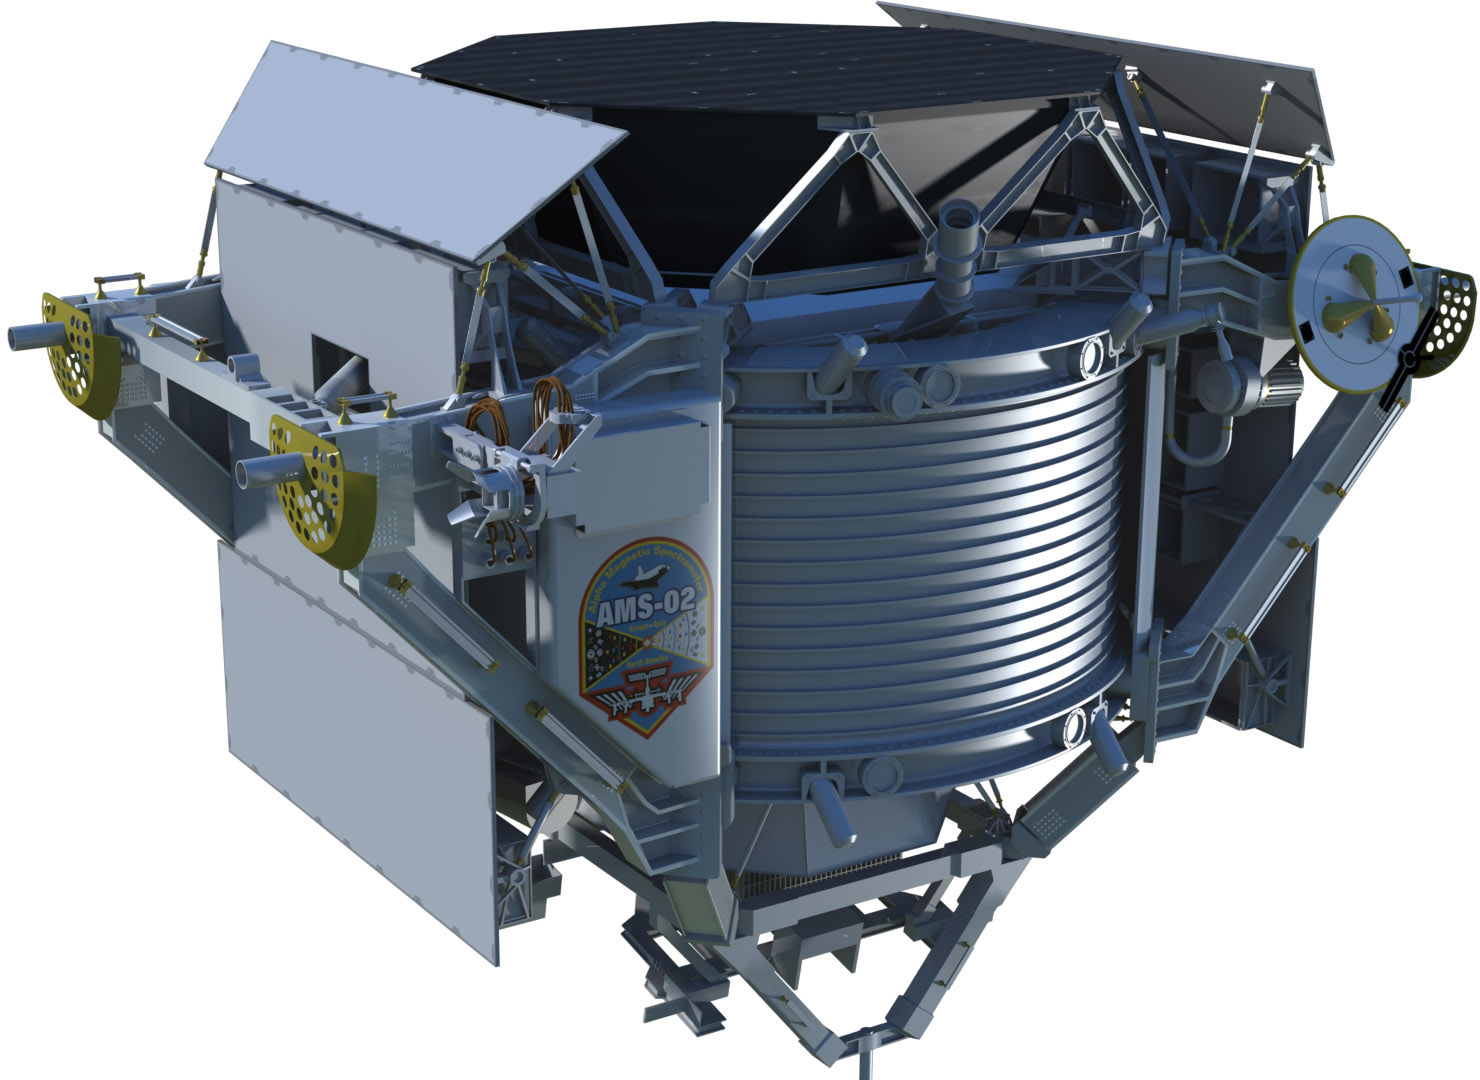
\includegraphics[width=0.30\textwidth]{satellite}
  \end{center}
  \vspace{-20pt}
\end{wrapfigure}
Mercoledì 3 Aprile 2013, è di portata storica per la Scienza. È il primo successo scientifico di AMS, il più potente e sensibile spettrometro magnetico galattico iper-freddo, appositamente concepito, costruito e messo in orbita sulla Stazione Spaziale Internazionale (Iss) a 400 Km di quota, per la ricerca di Antimateria e Materia Oscura nel Cosmo. AMS è un rivelatore di particelle, pesante otto tonnellate. Il progetto è stato realizzato da una collaborazione di 600 scienziati di 16 Paesi e 60 Istituzioni. L’ideatore e coordinatore del progetto è il premio Nobel Samuel Ting (MIT – CERN), il vice responsabile è lo scienziato italiano Roberto Battiston, fisico dell’Infn . AMS ha effettivamente osservato un “eccesso” di positroni (elettroni di carica positiva, cioè Antimateria) nel flusso di raggi cosmici provenienti dallo spazio profondo.L’esperimento AMS, installato sulla Iss grazie al volo dello Space Shuttle STS--134 Endeavour (l’ultima missione della navetta Usa, il 16 Maggio 2011) con a bordo il nostro astronauta Roberto Vittori, è concepito per catturare e studiare queste particelle prima che esse interagiscano con l’atmosfera terrestre, il nostro scudo vitale, perdendo così informazioni importanti sulla loro natura.

\section*{Osservazioni}
\label{osservazioni}

\emph{AMS--02 è uno spettrometro magnetico di grandi dimensioni realizzato per operare nello spazio. Tra le tante sfide del progetto, la principale è stata quella di mettere a punto un sistema magnetico in grado di lavorare nello spazio in sicurezza e per un periodo prolungato}.

La Collaborazione di AMS ha sviluppato due magneti:

\begin{itemize}
\item Un \textbf{magnete permanente} (Permanent Magnet, PM) che opera a temperatura ambiente. Il PM è composto da 6000 blocchi in lega di Neodimio accuratamente magnetizzati e poi incollati assieme. Questo magnete è stato già utilizzato nel prototipo di AMS, AMS--01, che ha volato nella missione Shuttle STS--91 nel 1998.

\item Un \textbf{magnete superconduttore} (Superconducting Magnet, SCM) in grado di operare a una temperatura di 4 gradi sopra lo zero assoluto (0 K). Il SCM è composto da 14 bobine di materiale superconduttore avvolte su una robusta struttura d’alluminio. La corrente che circola permanentemente nelle bobine genera al centro di AMS un campo magnetico fino a 0.87 Tesla di intensità. Per essere mantenuto alla bassissima temperatura di lavoro, il SCM necessita di un continuo raffreddamento realizzato tramite un contatto termico con una grande massa di elio superfluido (2500 litri) alla temperatura di 1.8 Kelvin. Il magnete superconduttore è stato testato nel large space simulator al centro ESA, ESTEC di Nordwijk in Olanda nell’aprile del 2010 dando buoni risultati.

\end{itemize}

Entrambi i sistemi magnetici hanno la stessa configurazione del campo, il cosiddetto anello magico, che assicura al magnete un momento di dipolo netto trascurabile e impedisce che, una volta installati nello spazio, ci siano accoppiamenti con il campo magnetico terrestre, cosa che disturberebbe l’orbita della Stazione Spaziale. I due magneti hanno anche dimensioni simili e presentano le stesse interfacce con i rivelatori dell’esperimento, sono quindi meccanicamente intercambiabili.

\textbf{L’elettronica} di AMS è una sfida tecnologica a sè stante. Lo spazio è infatti un ambiente estremamente ostile per le apparecchiature elettroniche data la presenza della radiazione cosmica. L’elettronica di AMS consta di oltre 600 diversi computer dotati di chip tolleranti alla radiazione, sviluppati appositamente per la fisica delle alte energie, circa 10 volte più veloci dei normali computer.

I risultati acquisiti da AMS, perfettamente in accordo con i modelli matematici e fisici più accreditati nel Modello Standard, sono fondati sull’osservazione di 25 miliardi di eventi che includono il rilevamento di 400mila positroni, di energia compresa tra 0.5 e 350 GigaelettronVolt (GeV), sul totale di 6.8 milioni di particelle osservate nell’intervallo energetico, nel corso del primo anno e mezzo di attività, dal 19 Maggio 2011 al 10 Dicembre 2012. È la prima scoperta da World Guinness Record dell’esperimento AMS. I dati acquisiti, infatti, rappresentano la più estesa collezione di particelle di Antimateria mai osservata e registrata prima nello spazio. Il primo “set” di positroni incrementa considerevolmente nell’intervallo di energia tra 10 e 250 GeV, con una curva piuttosto pronunciata di dati che poi diminuisce di un ordine di grandezza al di sopra del range 20--250 GeV. I dati non mostrano sostanziali variazioni significative nello spaziotempo: il flusso energetico di anti-particelle giunge da ovunque lo si osservi senza direzioni preferenziali. I risultati di AMS sono consistenti e in buon accordo, secondo gli scienziati, con il comportamento dei positroni prodotti dall’annichilazione di particelle di Materia Oscura nello spazio cosmico. Ma i dati finora acquisiti non sono ancora sufficienti per escludere altre spiegazioni.

\end{document}